\documentclass[onecolumn, draftclsnofoot,10pt, compsoc]{IEEEtran}
\usepackage{graphicx}
\usepackage{float}
\usepackage{url}
\usepackage{setspace}
\usepackage{caption}
\graphicspath{ {images/} }

\usepackage{geometry}
\geometry{textheight=9.5in, textwidth=7in}

\def \CapstoneTeamName{		Look Boss, No Hands}
\def \CapstoneTeamNumber{		9}
\def \GroupMemberOne{			Brandon Dring}
\def \GroupMemberTwo{			Nipun Bathini}
\def \GroupMemberThree{			Carl Benson}
\def \CapstoneProjectName{		CDK Global: No more touch. No more Keyboard. Bring it All Together. Using Technology to Teach Humans.}
\def \CapstoneSponsorCompany{	CDK Global}
\def \CapstoneSponsorPerson{		Trevor Moore}


\def \DocType{Fall Term - Project Report}

\newcommand{\NameSigPair}[1]{\par
\makebox[2.75in][r]{#1} \hfil 	\makebox[3.25in]{\makebox[2.25in]{\hrulefill} \hfill		\makebox[.75in]{\hrulefill}}
\par\vspace{-12pt} \textit{\tiny\noindent
\makebox[2.75in]{} \hfil		\makebox[3.25in]{\makebox[2.25in][r]{Signature} \hfill	\makebox[.75in][r]{Date}}}}

%%%%%%%%%%%%%%%%%%%%%%%%%%%%%%%%%%%%%%%
\begin{document}
\begin{titlepage}
    \pagenumbering{gobble}
    \begin{singlespace}
        \hfill
        \par\vspace{.2in}
        \centering
        \scshape{
            \huge CS Senior Capstone \DocType \par
            {\large December 2nd, 2017}\par
            \vspace{.5in}
            \textbf{\Huge\CapstoneProjectName}\par
            \vspace{.5in}
              
            \vfill
            {\large Prepared for}\par
            \Huge \CapstoneSponsorCompany\par
            \vspace{5pt}
            {\Large\NameSigPair{\CapstoneSponsorPerson}\par}
            {\large Prepared by }\par
            Group\CapstoneTeamNumber\par
            % 5. comment out the line below this one if you do not wish to name your team
            \vspace{0.2cm}
            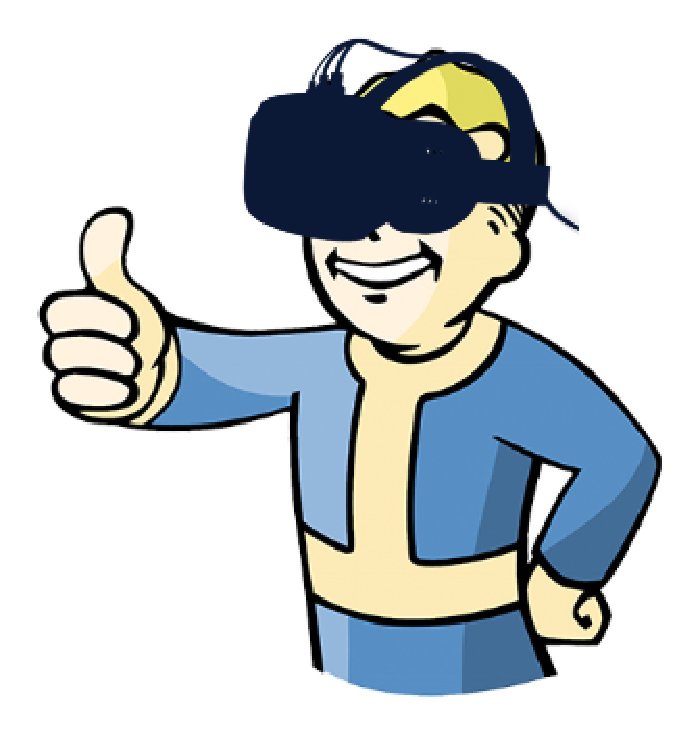
\includegraphics[height=4cm]{Team_logo}\\
            \vspace{0.2cm}
            \CapstoneTeamName\par
            \vspace{5pt}
            {\Large
                \NameSigPair{\GroupMemberOne}\par
                \NameSigPair{\GroupMemberTwo}\par
                \NameSigPair{\GroupMemberThree}\par
            }
            \vspace{20pt}
        }
        \begin{abstract}
        % 6. Fill in your abstract
        	This document seeks to explain what exactly we have been doing for the past 10 weeks with regards to the Look Boss, No Hands project. We will go over exactly what the project is trying to accomplish, and the weekly status updates on progress that lead up to where we are now. Then, a short excerpt talking about where the project is in its current form. Afterwards we will explain any problems we have encountered so far, and any interesting findings so far. Lastly, we will go over a retrospective on what we{'}ve done as a team this semester, and ways we can improve. 



        \end{abstract}
    \end{singlespace}
\end{titlepage}
\newpage
\pagenumbering{arabic}
\tableofcontents
\clearpage

\section{Project Purpose and Goals}
    Look Boss, No hands seeks to develop a new interaction method between a user looking at enterprise data. Instead of sitting behind a computer screen typing and clicking around to get graphs, and charts. This project aims to remove the standard methods of input, in lieu of more novel methods of input such as, voice and virtual reality. Using new pieces of hardware taking over the technology industry, a user should be able to tell a Alexa what they want to see, and have it displayed for them in VR to interact with

\section{Weekly Progress}
    \subsection{Week 2: Housekeeping, introductions, client meeting planning}
    
        \subsubsection{Overall}
            Week 2 was the week that we received our project assignments. We set up a Slack channel to maintain communication and invited our client to it as well. Brandon had created the Github for all the project related stuff, along with Google drive for sharing. We were in contact with our client and scheduled a time to have a face-to-face meeting the next week.
    
    \subsection{Week 3: Client meeting, Team Meeting, Problem Statement}
    
        \subsubsection{Client}
            Week 3 featured a meeting with our client and the rough draft of the problem statement. We met with our client for lunch and went over more details of the project as well as discussed what technologies we would be using, along with the hardware required. We also set up a recurring, weekly meeting over WebEx to keep our client up to date with current progress.
            
        \subsubsection{Writing}
            We finished and submitted the rough draft for the problem statement. In the problem statement, our description of the problem was that there are many new types of devices being introduced that lacked a connection between them. 
    
    
    \subsection{Week 4: AWS setup, create Alexa, Lambda, Problem statement}
        \subsubsection{Writing}
            Week 4 included the submission of our final draft for the problem statement as well as the beginning of experimentation with custom Alexa commands. We took the feedback from the rough draft as well as additional proofreading to fine tune the final draft for submission
        \subsubsection{Project}
            Brandon had set up the first instances of accounts allowing for the creation of Alexa skills and processing. 
    
    \subsection{Week 5: Requirements Document, Alexa and AWS }
    
        \subsubsection{Overall}
            Week 5 was the week we begin the requirements document in addition to beginning investigation into created custom Alexa skills. We each created a simple new command for Alexa to acknowledge and respond to. 
            
        \subsubsection{Writing}
            We wrote the rough draft for the requirements document. In the requirements document we went over more in depth details, specific requirements, and other non-functional requirements. The rough draft was sent to our client for feedback and approval.
            
        \subsubsection{Project}
            Alexa and AWS lambda were also programmed to connect to the remote server and get some data and return it. 
            
    
    \subsection{Week 6: Requirements document, TravisCI, Refactor, Socket.IO}
        \subsubsection{Writing}
            Week 6 was similar to the previous week. We revised our requirements document based on provided feedback and received client approval. We continued our work with custom Alexa commands, increasing functionality through more recognized phrases.
            
        \subsubsection{Project}
            Created ability to connect websockets on the remote server and have them broadcast messages to local laptop.
            Created continuous integration testing on Github for each new commit and PR.
            Refactored AWS files and folders to be  more modular and readable. 
            
    
    \subsection{Week 7: Tech Review, VR headsets}
    
        \subsubsection{Overall}
            Week 7 primarily focused on each of us beginning our technology review document. Brandon reviewed options for server coding language, graphics engine, and network communication framework. Nipun reviewed options for virtual assistants, data storage, and wearables. Carl reviewed options for VR headsets, data hosting services, and machine learning frameworks. 
            
        \subsubsection{Project}
            Client had received VR headsets, implemented basic game in Unity in VR to play with blocks and throw them around. 
    
    \subsection{Week 8: Agile adoption, MongoDB mock data }
    
        \subsubsection{Writing}
            Week 8 featured the editing and submission of the final drafts of our technology reviews. We took the feedback we each received from the in-class peer review to identify the areas we needed to make changes. 
            
        \subsubsection{Project}
            Everyone created agile stories for tasks relating the project. 
            Defined sprint lengths, and set up more regular meeting times and demos for the project with client.
            Created script to create mock sales data to be used in VR later on in the project.
            
    \subsection{Week 9: Unique Alexa commands}
    
        \subsubsection{Project}
            Week 9 was the week we began our Agile development. Brandon setup Zenhub to add, track, and assign stories. The stories for this sprint were:
            \begin{itemize}
                \item Nipun created a comprehensive README for both the Alexa and AWS server setup as well as created Mocha tests for basic server routes.
                \item Carl researched machine learning frameworks for providing more human-like responses from Alexa as well as created a Python script for the generation of fake sales data.
                \item Brandon created a basic VR environment in Unity as well as looked into the implementation of RabbitMQ in Unity. 
            \end{itemize}
            
            \vspace{10pt}            
            
            Created unique Alexa commands by registering variables in the sample utterances that later tell the server what route to get and what data to query. 
            
            
    
    \subsection{Week 10: Sprints, Progress report, design doc}
        
        \subsubsection{Writing}
            Week 10 included the writing of the design document and the progress report. The design document detailed the design and implementation details, as well as information on the components of the system from multiple viewpoints.
            
            \vspace{10pt}
            
            The other task we worked on this week was the progress report, which covers what we accomplished this past term in the form of a written report and a recorded presentation. 
            
    
    
\section{Where We Are}
	Currently we have set up the skeleton framework of our project, meaning that we have have created a functional Alexa account that can take in basic commands and phrases. We have also a pretty solid understanding as how to modify and add onto what we currently have with the Alexa to add more commands and use speech variables within our sample utterances.
	
	\vspace{10pt}

    On top of that, we have a functional Lambda service inside AWS that the Alexa speech processing maps to. From there we have configured certain routes to use variables dictated by the speech patterns received by the Alexa and go to the respective server routes to query the correct data. Along with querying routes on the server, there is also semi-intelligent responses whether an error was encountered or Alexa/Lambda couldn{'}t understand the request. 
    
    \vspace{10pt}
    
    As for the VR side of things, it wasn{'}t until about a month ago that we actually had a VR headset in hand to begin development. But since acquiring the headset, we have researched packages to use to fit our needs and implemented it into a working skeleton platform. We have found a very helpful package called VRTK that helps abstract away all the complexity of the math and physics that goes into creating a VR experience. As such, we currently have a VR environment where the user can move around and teleport, interact with objects and get logical feedback regarding physics, and even climb trees. We have also connected the local VR headset up to the AWS server, so that the commands received from the Alexa eventually make its way all the way down to the local headset. 


\section{Problems, and solutions}

    One issue we ran into was waiting for the hardware 
    \begin{itemize}
        \item Waiting for the Alexa was not that bad, and we received them on October 18th.  
        \item But waiting for the HTC Vive until the middle of November, made it difficult for us to begin to get a start on the VR side 
    \end{itemize}
    
    \vspace{10pt}
    
    We also did not all setup Zenhub, until the start of November, and assigning tasks has been much simpler since.
    
    \vspace{10pt}
    
    The client had also requested Alexa seem non-robotic, thus the responses shouldn{'}t all be hardcoded and Alexa should provide useful suggestions to the user. 
    
    \begin{itemize}
        \item This makes us think of using another AWS service for machine learning, or switching part of the project over to Python to use some of their famous AI/Machine Learning libraries.
    \end{itemize}
    
    \vspace{10pt}
    
    Using something simple in VR like data visualization has already been done. But the package/asset requires money to buy. 
    
    \begin{itemize}
        \item We{'}re stuck at either developing our own data visualization library, or convincing the client to buy some. 
    \end{itemize}
    
    \vspace{10pt}
    
    The amount of writing that has been required by the class so far has taken away from the time to actually build the project
    
    \begin{itemize}
        \item Significant work will be implemented over the course of winter break to make up for lost time during fall term.
    \end{itemize}
    
    \vspace{10pt}
    
    Instead of sharing an AWS account (which requires a credit card), to avoid others seeing private financial information. We have all had to create separate AWS accounts and clone the code from Github and paste it into whatever AWS service we need. 
    
    \begin{itemize}
        \item As a solution, I might be able to open up an AWS account since it is free for 12 months with a prepaid credit card that I has \$3 on it. Then everyone can share the same account and not worry about copy and pasting code. 
    \end{itemize}



\section{Interesting Code}
    The way that the Alexa SDK is set up inside AWS is really quite ingenious, allowing for rapid development and quick modifications.

    \begin{figure}
        \centering
        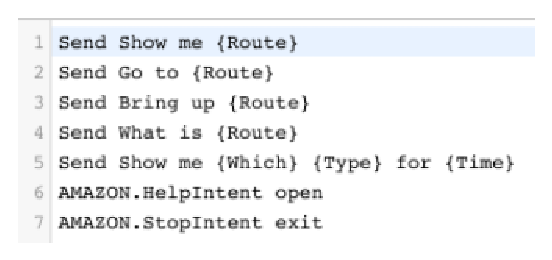
\includegraphics[width=0.5\textwidth]{alexa-phrases.eps}
        \caption{Sample Alexa utterance list}
        \label{fig:alexa}
    \end{figure}

    For example, figure ~\ref{fig:alexa} shows how you specify to Alexa what commands to listen for within your custom Alexa skill. The first word is the intent type/name, the following words after that are the exact commands that Alexa listens for. The values wrapped in {‘}\{\}{’} are variables which you can assign any value, which are later passed into an object with the key Route along with whatever value filled in the variable Route. 
    
    The Unity package that we had found was also really neat as well, VRTK allows for simple drag-and-drop attributes onto objects within the VR environment. Where you search for the functionality that you desire, and drag it onto the GameObject you want. There is no longer a need for computing angular velocity when throwing an object or dropping it. 

    \begin{figure}
        \centering
        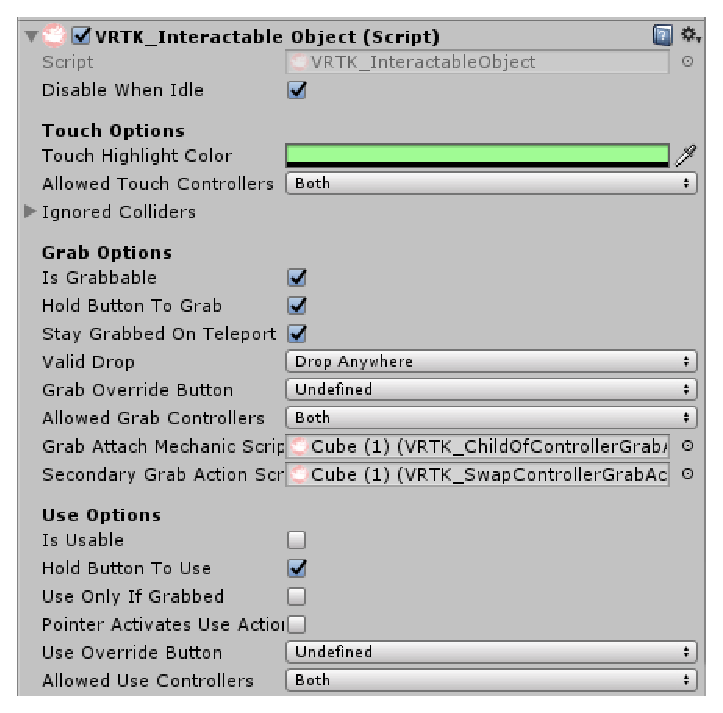
\includegraphics[width=0.5\textwidth]{VRTK.eps}
        \caption{Object attributes with VRTK}
        \label{fig:vrtk}
    \end{figure}

    Figure ~\ref{fig:vrtk} shows the attributes put onto a cube, and the added options of it being grabbable and usable. This package allows us to not reinvent the wheel, and use something that is probably both more reliable and efficient when it comes to VR interactions.


\section{Retrospective}
    \begin{tabular}{| p{0.3\linewidth} | p{0.3\linewidth} | p{0.3\linewidth} |}
        \hline 
        Positives & Negatives & Actions \\ \hline
        
        All pieces of required hardware were received & Lack of planning and forethought with regards to Agile throughout start of semester & Creating future tasks, breaking them down into respectable size, and greater accountability between group members for project tasks \\ \hline
        
        All necessary software frameworks were set up & Separate AWS accounts & Create a shared AWS using pre-paid credit card \\ \hline
        
        Significant contribution from all regarding group writing assignments & Sharing single VR headset & Brandon bought a personal Oculus Rift during Black Friday \\ \hline
        
        Base functionality of all aspects of the project were completed & Difficult to demo for client & Pre-record demos to be posted to Google Drive or ENGR webspace \\ \hline

        
    \end{tabular}

\end{document}